\RequirePackage{fix-cm}
\documentclass[10pt]{article}
\usepackage[letterpaper,margin=0.2in]{geometry}
\usepackage{amsmath,amssymb,bm}
\newcommand{\ind}{\mathbb{I}}
\usepackage{multicol}
\usepackage{graphicx}
\usepackage{enumitem}
\usepackage{titlesec}
\usepackage{tabularx}
\usepackage{tikz}

\setlength{\parindent}{0pt}
\setlength{\columnsep}{8pt}
\setlength{\columnseprule}{0.2pt}
\setlist{nosep,leftmargin=*}
\titleformat*{\section}{\large\bfseries\raggedright}
\titleformat*{\subsection}{\normalsize\bfseries}
\titlespacing*{\section}{0pt}{3pt}{1pt}
\titlespacing*{\subsection}{0pt}{2pt}{0pt}
\AtBeginDocument{\setlength{\abovedisplayskip}{2pt}\setlength{\belowdisplayskip}{2pt}\setlength{\abovedisplayshortskip}{0pt}\setlength{\belowdisplayshortskip}{1pt}}
\setlength{\jot}{1pt}
\pagestyle{empty}

\newcommand{\vx}{\mathbf{x}}
\newcommand{\vw}{\mathbf{w}}
\newcommand{\vt}{\mathbf{t}}
\newcommand{\vu}{\mathbf{u}}
\newcommand{\vv}{\mathbf{v}}
\newcommand{\vr}{\mathbf{r}}
\newcommand{\cE}{\mathcal{E}}
\newcommand{\cL}{\mathcal{L}}
\newcommand{\sub}[1]{\textit{#1}:}  % in-line sub-label (Def/Effect/Cause/Fix/Rule/Why...)
\newcommand{\va}{\mathbf{a}}
\newcommand{\vb}{\mathbf{b}}
\newcommand{\vz}{\mathbf{z}}
\newcommand{\vy}{\mathbf{y}}

\begin{document}
\fontsize{5.5}{6.4}\selectfont
\raggedcolumns
\begin{multicols*}{3}

\section{Limitations of Linear Models}
\textbf{Linear boundary}: \sub{Def} a linear classifier (LogReg, perceptron, softmax pairwise) predicts by the sign of $z=\vw^T\vx+b$ ($\sigma(z)\ge0.5\iff z\ge0$) $\to$ boundary is the hyperplane $\{\vx:\vw^T\vx+b=0\}$.\\
\textbf{Linearly separable} \sub{Def} two sets of points are linearly separable if there exists a hyperplane that perfectly separates them. \sub{Effect if not} no linear classifier reaches 100\% training accuracy, no matter how much data or which optimizer.\\
\textbf{Half-space} \sub{Def} $H=\{\vx\in\mathbb R^d:\mathbf c^T\vx+b\ge0\}$ ($\mathbf c\in\mathbb R^d$, $b\in\mathbb R$) = all points on one side of a hyperplane; $\{\mathbf c^T\vx+b=0\}$ is the hyperplane itself.\\
\textbf{Convex set} \sub{Def} $S\subseteq\mathbb R^d$ is convex if $\forall\vx^{(a)},\vx^{(b)}\in S$, $\forall\lambda\in[0,1]$: $\lambda\vx^{(a)}+(1-\lambda)\vx^{(b)}\in S$ (the segment between any 2 points of $S$ stays in $S$).\\
\textbf{Half-space is convex} \sub{Proof} $\vx^{(a)},\vx^{(b)}\in H$, $\lambda\in[0,1]$, split $b=\lambda b+(1-\lambda)b$:
\begin{align*}
&\mathbf c^T(\lambda\vx^{(a)}+(1-\lambda)\vx^{(b)})+b\\
&=\lambda(\mathbf c^T\vx^{(a)}+b)+(1-\lambda)(\mathbf c^T\vx^{(b)}+b)\ge0
\end{align*}
\textbf{XOR}: $t=1$ iff $x_1\ne x_2$: $(0,0)\!\to\!0$, $(0,1)\!\to\!1$, $(1,0)\!\to\!1$, $(1,1)\!\to\!0$. \sub{Theorem} not linearly separable.\\
\textbf{Algebraic proof} (XOR): \sub{Constraints} $t=1\Rightarrow b+w_1x_1+w_2x_2\ge0$; $t=0\Rightarrow b+w_1x_1+w_2x_2<0$:\\
$(0,0)$: $b<0$;\ \ $(0,1)$: $b+w_2\ge0$;\ \ $(1,0)$: $b+w_1\ge0$;\ \ $(1,1)$: $b+w_1+w_2<0$.\\
\sub{Contradiction} add the 2 positive constraints: $2b+w_1+w_2\ge0$; Add the 2 negative ones: $2b+w_1+w_2<0$.\\
\textbf{Geometric proof} \sub{Steps} (any dataset, by contradiction):\\
(1) Find 2 class-1 points $A,C$ and 2 class-0 points $B,D$ whose segments $\overline{AC}$, $\overline{BD}$ intersect.\\
(2) Intersection $F$: solve $\lambda A+(1-\lambda)C=\mu B+(1-\mu)D$ (2 eqs, 2 unknowns), check $\lambda,\mu\in[0,1]$. \sub{Shortcut} if $\frac{A+C}{2}=\frac{B+D}{2}$ then $F$ = that midpoint.\\
(3) Assume separable: $\exists f(\vx)=\vw^T\vx+b$ with class 1 in $H^+=\{\vx:f(\vx)\ge0\}$, class 0 in $H^-=\{\vx:f(\vx)<0\}$.\\
(4) $H^+$, $H^-$ are half-spaces $\Rightarrow$ convex.\\
(5) $A,C\in H^+$ and $H^+$ convex $\Rightarrow\overline{AC}\subseteq H^+\Rightarrow F\in H^+$.\\
(6) $B,D\in H^-$ and $H^-$ convex $\Rightarrow F\in H^-$.\\
(7) $H^+\cap H^-=\emptyset$, $F$ can't be in both $\Rightarrow$ contradiction $\Rightarrow$ not linearly separable.\ $\square$\\
\sub{Why (5), algebraically} $f$ affine $\Rightarrow f(F)=\lambda f(A)+(1-\lambda)f(C)\ge0$, but also $f(F)=\mu f(B)+(1-\mu)f(D)<0$. (Algebraic proof = this at the midpoint $F$.)\\
\sub{Variant} a class-0 point $P$ lies on a class-1 segment ($P=\lambda A+(1-\lambda)C$, 3 collinear points) or inside a class-1 triangle $\Rightarrow f(P)\ge0$, contradicts $P\in H^-$.\\
\sub{Intuition} separable $\iff$ the convex hulls of the 2 classes don't intersect.\\
\textbf{Feature map} \sub{Fix} add $x_3=\phi(\vx)$ (e.g.\ $x_1x_2$, $x_j^2$) so the classes become separable in the extended space; Boundary is linear in $(x_1,x_2,x_3)$, nonlinear after substituting $x_3=\phi(\vx)$ back.\\
\sub{Steps} pick $\phi$ on which the classes differ $\to$ add the $x_3$ column to the table $\to$ pick $(b,\vw)$ satisfying every row's constraint $\to$ substitute $x_3=\phi(\vx)$ for the original-space boundary.\\
\sub{XOR} $x_3=x_1x_2$, $(b,w_1,w_2,w_3)=(-0.5,1,1,-2)$ $\to$ $x_1+x_2-2x_1x_2-0.5=0\iff(2x_1-1)(2x_2-1)=0$ $\to$ lines $x_1=0.5$, $x_2=0.5$.\\
\sub{Cons} needs domain knowledge + manual experimentation; \#features grows combinatorially ($d$ inputs $\to O(d^2)$ degree-2 products); Overfits without regularization.\\
\textbf{Motivation for NN}: learn the features from data instead of hand-crafting them; Last layer of a NN = linear classifier on learned features, $\vw^T\phi(\vx)+b$.

\section{Introduction to Neural Networks}
\subsection{The Neuron}
\textbf{Artificial neuron} \sub{Def} $y=f(\vw^T\vx+b)$; $\vx$ = inputs (features), $\vw$ = weights (learned), $b$ = bias, $z=\vw^T\vx+b$ = pre-activation, $f$ = activation function (usually nonlinear), $y$ = output (activation).\\
\textbf{Biology map}: dendrites = input channels; Synapse = weight (strength \& sign, negative = inhibitory); Cell body = $\sum_jw_jx_j+b$ (integrates); Bias = intrinsic excitability; $f$ = whether/how strongly it fires; Axon = output channel.\\
\textbf{Output}: real-valued (like a firing rate), not binary (unless $f$ = threshold).\\
\textbf{Linear models as NN}: $f$ = identity $\to$ LinReg; $f=\sigma$ $\to$ LogReg = a single neuron; Softmax regression = 1-layer NN with $K$ output units, $\vy=\text{softmax}(W\vx+\vb)$. \sub{Cons} 1 affine map + activation $\to$ only linear boundaries.\\
\textbf{Network diagram}: node = a value, arrow = weighted connection; Computation (multiply, sum, bias, $f$) is implied, not drawn. \sub{Conventions} vertical/horizontal layout, inputs as nodes, bias as a node (= weight from a constant 1): same network, only the drawing changes. \textbf{Computation graph}: every numerical step explicit (used for backprop).

\subsection{MLP Definitions}
\textbf{Unit} \sub{Def} any node in a NN. \textbf{Neuron} \sub{Def} a unit that computes its output from its inputs. \sub{Contrast} input units only hold data (no computation) $\to$ units but not neurons.\\
\textbf{Input layer} \sub{Def} represents the input features; Does no computation.\\
\textbf{Computational layer} \sub{Def} a layer whose units are all neurons; Hidden + output layers are computational, the input layer is not.\\
\textbf{Output layer} \sub{Def} computational layer producing values with a defined interpretation (class probabilities / continuous value).\\
\textbf{Hidden layer} \sub{Def} any computational layer between the input and output layers; Its outputs = internal representations (learned features, not hand-designed; neither observed data nor final prediction).\\
\textbf{Feedforward NN} \sub{Def} computation flows only from earlier to later layers, no feedback loops (a DAG). \textbf{Recurrent NN} \sub{Def} has cycles (not in course).\\
\textbf{Fully connected layer} \sub{Def} each unit receives input from \emph{every} unit of the previous layer, and \emph{only} from those units (no skip edges).\\
\textbf{MLP} \sub{Def} feedforward NN with $\ge1$ hidden layers between input and output, every layer fully connected.\\
\textbf{Perceptron} \sub{Def} Rosenblatt's (1958) neuron, weighted sum + hard threshold; ``MLP'' name is historical (modern nets use smooth $f$).\\
\textbf{Inference} \sub{Def} computing the network's output for a given input. \textbf{Forward pass} \sub{Def} the computation doing it (input $\to$ output). \sub{Training} adds the loss $\cL(\va^{(M)},\vt)$ (needs known $\vt$); Forward pass + loss = phase 1 of backprop; All steps differentiable $\to$ trainable by GD.\\
\textbf{Roles}: hidden layers build intermediate features; Output layer turns them into a task-meaningful prediction.

\subsection{Counting Layers}
\textbf{Rule}: $M$ = \#layers = \#computational layers = \#hidden $+1$; \emph{Never} count the input layer.\\
\textbf{\#Neurons}: hidden + output units only; \textbf{\#Units}: also counts the input units.\\
\textbf{Layer of a neuron} (general DAG): input units = layer 0; Neuron's layer $=1+\max$(layers of the units feeding it) (longest path from the inputs).\\
\textbf{Naming}: LogReg / softmax = 1-layer NN (no hidden); ``2-layer NN'' = 1 hidden + output.\\
\textbf{Ex 1}: $4\to5\to3\to1$ = 3-layer MLP ($M=3$, 2 hidden layers, 9 neurons, 13 units).\\
\textbf{Ex 2}: inputs $A,B$; edges $A\!\to\!C$, $B\!\to\!C$, $A\!\to\!D$, $C\!\to\!D$, $D\!\to\!E$ $\to$ neurons $C,D,E$; Layers $C=1$, $D=2$, $E=3$ $\to$ 3 layers; Feedforward (no loops); $A\!\to\!D$ skips layer 1 $\to$ not fully connected $\to$ not an MLP.\\
\textbf{\#Params}: $\sum_{m=1}^M D^{(m)}(D^{(m-1)}+1)$ (weights $D^{(m)}D^{(m-1)}$ + biases $D^{(m)}$). \sub{Ex 1} $5(4\!+\!1)+3(5\!+\!1)+1(3\!+\!1)=47$.

\subsection{Notation \& Forward Pass}
{\fontsize{4}{4.7}\selectfont\setlength{\tabcolsep}{2pt}\renewcommand{\arraystretch}{0.95}%
\begin{tabularx}{\linewidth}{@{}l>{\raggedright\arraybackslash}p{0.27\linewidth}>{\raggedright\arraybackslash}X@{}}
\textbf{Symbol} & \textbf{Dim} & \textbf{Meaning}\\\hline
$M$ & scalar & \#computational layers\\
$m$ & $\{0,\dots,M\}$ & layer index: 0 input, $1..M\!-\!1$ hidden, $M$ output\\
$D^{(m)}$ & scalar & \#units in layer $m$\\
$\va^{(0)}=\vx$ & $D^{(0)}\times1$ & network input\\
$W^{(m)}$ & $D^{(m)}\times D^{(m-1)}$ & weights into layer $m$ (out $\times$ in)\\
$\vb^{(m)}$ & $D^{(m)}\times1$ & biases of layer $m$\\
$f^{(m)}$ & $\mathbb R\to\mathbb R$ & activation, element-wise (softmax: whole vector)\\
$\vz^{(m)}$ & $D^{(m)}\times1$ & pre-activations of layer $m$\\
$\va^{(m)}$ & $D^{(m)}\times1$ & activations of layer $m$\\
$\mathbf h^{(m)}=\va^{(m)}$ & $D^{(m)}\times1$ & hidden activations, $m\in\{1,\dots,M\!-\!1\}$\\
$\vy=\va^{(M)}$ & $D^{(M)}\times1$ & network output\\
$\vt$ & $D^{(M)}\times1$ & target\\
$\cL(\va^{(M)},\vt)$ & scalar & loss for one example
\end{tabularx}}\\
\textbf{Weight index}: $W^{(m)}_{j,k}$ = weight \emph{to} unit $j$ of layer $m$ \emph{from} unit $k$ of layer $m\!-\!1$ (1st index = receiver). \sub{Why $W\va$} $W^{(m)}$ is (out $\times$ in) $\to W^{(m)}\va^{(m-1)}\in\mathbb R^{D^{(m)}}$.\\
\textbf{Forward pass} ($m=1,\dots,M$):\\
\sub{Scalar}
\[ z^{(m)}_j=\textstyle\sum_{k=1}^{D^{(m-1)}}W^{(m)}_{j,k}a^{(m-1)}_k+b^{(m)}_j,\quad a^{(m)}_j=f^{(m)}(z^{(m)}_j) \]
\sub{Vectorized} $\vz^{(m)}=W^{(m)}\va^{(m-1)}+\vb^{(m)}$,\ \ $\va^{(m)}=f^{(m)}(\vz^{(m)})$\\
\sub{Loss} $\cL=\cL(\va^{(M)},\vt)$; Cost $\cE$ = average of $\cL$ over examples.\\
\textbf{Output layer} \sub{Why only vectorized} softmax is not element-wise: each $y_j$ depends on the whole $\vz^{(M)}$. \sub{Reg, 1 output} $f^{(M)}$ = identity, $y=z^{(M)}_1$.\\
\textbf{Inference} \sub{Steps} $\vz^{(1)}=W^{(1)}\vx+\vb^{(1)}$ $\to$ $\va^{(1)}=f^{(1)}(\vz^{(1)})$ (threshold: $z\ge0\to1$) $\to$ repeat per layer $\to$ softmax output $y_k=e^{z_k}/\sum_{k'}e^{z_{k'}}$ $\to$ predict $\arg\max_k y_k$; Label which values are input / hidden / output.\\
\textbf{Units affected by $W^{(m)}_{j,k}$}: only $z^{(m)}_j,a^{(m)}_j$ in layer $m$ (other units of layer $m$ and all earlier layers unchanged), then \emph{every} unit of layers $m\!+\!1,\dots,M$ (fully connected), then $\cL$. \sub{Equations to write} exactly those $z$'s, $a$'s and $\cL$, in forward order.

\subsection{Designing an MLP}
{\fontsize{4}{4.7}\selectfont\setlength{\tabcolsep}{2pt}\renewcommand{\arraystretch}{0.95}%
\begin{tabularx}{\linewidth}{@{}>{\raggedright\arraybackslash}p{0.36\linewidth}>{\raggedright\arraybackslash}X@{}}
\textbf{Decision} & \textbf{How chosen}\\\hline
\#input units & data representation ($D$ features; $28\times28$ image flattened $\to\vx\in\mathbb R^{784}$, 1 unit per pixel)\\
Target & one-hot $\vt\in\mathbb R^{K}$; class index from 0 $\to$ digit $k$ has 1 at entry $k\!+\!1$\\
\#hidden layers & hyperparameter (tune on val); \#comp.\ layers $=$ this $+1$\\
\#units per hidden layer & hyperparameter\\
Hidden activation & hyperparameter (default ReLU)\\
\#output units & task: Reg 1; Binary 1; $K$-class $K$\\
Output activation & task: Reg identity; Binary $\sigma$; $K$-class softmax
\end{tabularx}}\\[1pt]
{\fontsize{4}{4.7}\selectfont\setlength{\tabcolsep}{2pt}\renewcommand{\arraystretch}{0.95}%
\begin{tabularx}{\linewidth}{@{}lll>{\raggedright\arraybackslash}X>{\raggedright\arraybackslash}X@{}}
\textbf{Task} & $D^{(M)}$ & $f^{(M)}$ & \textbf{Target} & \textbf{Loss}\\\hline
Reg & 1 & identity & $t\in\mathbb R$ & SE $\frac12(y-t)^2$\\
Binary & 1 & $\sigma$ & $t\in\{0,1\}$ & CE\\
$K$-class & $K$ & softmax & one-hot $\vt\in\{0,1\}^K$ & CE $-\vt^T\log\vy$
\end{tabularx}}\\
\textbf{Softmax derivative}: $\frac{\partial y_i}{\partial z_j}=y_i(\ind[i=j]-y_j)$ ($i=j$: $y_i(1-y_i)$; $i\ne j$: $-y_iy_j$). \sub{With CE} $\frac{\partial\cL}{\partial\vz}=\vy-\vt$.

\subsection{Activation Functions}
\textbf{Activation function} \sub{Def} $f:\mathbb R\to\mathbb R$, typically a nonlinear scalar function, applied element-wise to $\vz^{(m)}$: $\va^{(m)}=f(\vz^{(m)})$. \sub{Exception} softmax (output layer, $K$-class) acts on the whole vector, still called an activation function.\\
\textbf{Sigmoid}: $\sigma(z)=\frac1{1+e^{-z}}\in(0,1)$; $\sigma'=\sigma(1-\sigma)\le0.25$ (max at $z=0$).\\
\textbf{Tanh}: $\tanh(z)=\frac{e^z-e^{-z}}{e^z+e^{-z}}=2\sigma(2z)-1\in(-1,1)$; $\tanh'=1-\tanh^2\le1$ (max at $z=0$). \sub{Shape} sigmoid compressed $\times2$ horizontally, stretched $\times2$ vertically, shifted down 1 $\to$ passes through origin, odd (symmetric about origin).\\
\textbf{ReLU}: $\max(0,z)\in[0,\infty)$; $\text{ReLU}'=\ind[z>0]$ (not differentiable at $z=0$; define 0 or 1, doesn't affect training). \sub{Nonlinearity} only the kink at $z=0$, but enough for expressive power.\\
\textbf{Threshold}: $\ind[z\ge0]\in\{0,1\}$ ($f(0)=1$); Derivative 0 for $z\ne0$, undefined at 0.\\
\begin{minipage}{\linewidth}
\textbf{Graphs}: dashed lines at $\pm1$; $\sigma$ saturates at 0 / 1, tanh at $-1$ / 1; Threshold: open circle $(0,0)$, filled $(0,1)$.\\[1pt]
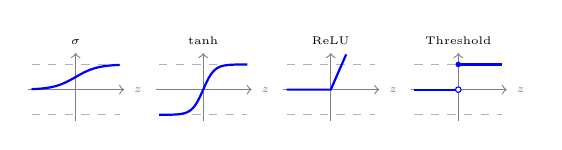
\begin{tikzpicture}[x=0.14cm,y=0.32cm,font=\fontsize{4}{4}\selectfont]
\foreach \i/\name in {0/$\sigma$,1/$\tanh$,2/ReLU,3/Threshold}{
  \begin{scope}[xshift=\i*1.62cm]
  \draw[gray,->] (-4.3,0)--(4.4,0) node[right]{$z$};
  \draw[gray,->] (0,-1.25)--(0,1.45);
  \draw[gray!60,dashed] (-4,1)--(4,1) (-4,-1)--(4,-1);
  \node[above] at (0,1.4) {\name};
  \end{scope}}
\draw[blue,thick,domain=-4:4,samples=40] plot (\x,{1/(1+exp(-\x))});
\begin{scope}[xshift=1.62cm]\draw[blue,thick,domain=-4:4,samples=40] plot (\x,{tanh(\x)});\end{scope}
\begin{scope}[xshift=3.24cm]\draw[blue,thick] (-4,0)--(0,0)--(1.4,1.4);\end{scope}
\begin{scope}[xshift=4.86cm]\draw[blue,thick] (-4,0)--(0,0) (0,1)--(4,1);
  \draw[blue,fill=white] (0,0) circle (0.25pt*4); \fill[blue] (0,1) circle (0.25pt*4);\end{scope}
\end{tikzpicture}
\end{minipage}\\
\textbf{Why nonlinear $f$}: without it stacked linear layers collapse to 1 linear map; $f$ is the only source of nonlinearity.\\
\textbf{Saturated} \sub{Def} $f$ flat when $z$ far from 0 $\to$ a small change in incoming weights barely changes the output.\\
\textbf{Dead neuron} \sub{Def} GD stops updating a neuron's incoming weights because $f'\approx0$ at the inputs it receives (even if its output is wrong; any depth).\\
\textbf{Vanishing gradient} \sub{Def} the deeper the net, the smaller the gradients for early-layer weights. \sub{Cause} chain rule gives one $f'$ factor per layer between the weight and the output; Factors $<1$ $\to$ product shrinks exponentially. \sub{Effect} early layers learn slowly / not at all.\\
\textbf{Zero-centred} \sub{Def} activations can be positive or negative (tanh).\\
\textbf{Dying ReLU} \sub{Def} $z<0$ for every training input $\to$ always outputs 0, incoming weights never update. \sub{Fix} Leaky ReLU / ELU (small nonzero output for $z<0$).\\
\textbf{Sigmoid all-positive}: \sub{Effect} next layer's inputs all $>0$ $\to$ each update increases all or decreases all of a unit's incoming weights $\to$ zigzag, slow. \sub{Fix} tanh (zero-centred).\\
{\fontsize{4}{4.7}\selectfont\setlength{\tabcolsep}{2pt}\renewcommand{\arraystretch}{0.95}%
\begin{tabularx}{\linewidth}{@{}l>{\raggedright\arraybackslash}p{0.25\linewidth}>{\raggedright\arraybackslash}p{0.18\linewidth}>{\raggedright\arraybackslash}X@{}}
 & \textbf{GD} & \textbf{Dead neuron} & \textbf{Vanishing grad}\\\hline
Sigmoid & Yes: diff.\ $\forall z$ & No: $f'\ne0$ & Yes: $f'\to0$ for $|z|$ large\\
Tanh & Yes: diff.\ $\forall z$ & No: $f'\ne0$ & Yes: $f'\to0$ for $|z|$ large\\
ReLU & Yes: diff.\ except $z=0$ & Yes: $f'=0$ for $z<0$ & No: $f'=1$ for $z>0$\\
Threshold & No: $f'=0$ a.e. & Yes: $f'=0$ & Yes: $f'=0$ a.e.
\end{tabularx}}\\
\textbf{Poor-gradient inputs}: $\sigma$, tanh: $|z|$ large; ReLU: $z<0$.\\
\textbf{Sigmoid Pros}: smooth, everywhere-differentiable approximation of threshold ($\to$ GD works); Output = firing probability.\\
\textbf{ReLU Pros}: cheap (one comparison); Near-linear (identity for $z>0$) $\to$ easy to optimize; Slope 1 $\to$ no vanishing gradient $\to$ enables deep nets.\\
\textbf{Choice} (hyperparameter, hidden \& output chosen separately; judged by how well GD trains $\to$ Idea \#1 Learning is optimization): \sub{Hidden} must be nonlinear + support GD; ReLU default; Tanh if zero-centred matters; Sigmoid rarely. \sub{Output} by task (identity / $\sigma$ / softmax: interpretable output matching the loss). \sub{Threshold} only for perceptron history \& hand-picked weights.

\section{Expressiveness of Neural Networks}
\textbf{Linear activations collapse}: $f$ = identity $\Rightarrow\vy=W^{(2)}(W^{(1)}\vx+\vb^{(1)})+\vb^{(2)}=W_{eq}\vx+\vb_{eq}$,
\[ W_{eq}=W^{(2)}W^{(1)},\quad \vb_{eq}=W^{(2)}\vb^{(1)}+\vb^{(2)} \]
\sub{Affine $f(z)=az+c$} (per neuron, $A=\operatorname{diag}(\mathbf a)$, $\mathbf c$ stacked): $W_{eq}=W^{(2)}AW^{(1)}$, $\vb_{eq}=W^{(2)}(A\vb^{(1)}+\mathbf c)+\vb^{(2)}$ $\to$ still linear. \sub{Effect} any depth of linear layers = 1 linear layer (= LinReg).\\
\textbf{Threshold unit} ($f(z)=\ind[z\ge0]$, $x_j\in\{0,1\}$) \sub{Templates}\\
AND $f(x_1\!+\!x_2\!-\!1.5)$; OR $f(x_1\!+\!x_2\!-\!0.5)$; NOT $f(-x_1\!+\!0.5)$; NAND $f(-x_1\!-\!x_2\!+\!1.5)$; $x_1\wedge\neg x_2$: $f(x_1\!-\!x_2\!-\!0.5)$.\\
\sub{How $\vw,b$ decide} $w_j>0$: $x_j=1$ pushes toward 1; $w_j<0$: needs $x_j=0$; $b$ = threshold (how many conditions must hold). $\vw$ = normal of the boundary, points to the class-1 side.\\
\sub{Steps to hand-pick} truth table $\to$ plot the 4 points $\to$ draw a separating line $\to$ write it as $\vw^T\vx+b=0$, sign chosen so the class-1 side is $\ge0$ $\to$ verify every row.\\
\textbf{XOR, 2-layer}:\\
\sub{(a)} $x_1\oplus x_2=(x_1\wedge\neg x_2)\vee(\neg x_1\wedge x_2)$: $h_1=f(x_1-x_2-0.5)$, $h_2=f(-x_1+x_2-0.5)$, $y=f(h_1+h_2-0.5)$.\\
\sub{(b)} $x_1\oplus x_2=(x_1\vee x_2)\wedge\neg(x_1\wedge x_2)$: $h_1=f(x_1+x_2-0.5)$ (OR), $h_2=f(-x_1-x_2+1.5)$ (NAND), $y=f(h_1+h_2-1.5)$ (AND).\\
\textbf{Row detector}: unit fires iff $\vx=\vx^{(i)}$: $w_j=+1$ if $x^{(i)}_j=1$, $-1$ if $x^{(i)}_j=0$; $b=-(\#\text{1s in }\vx^{(i)})+0.5$. \sub{Why} $\vw^T\vx\le\#\text{1s}$, equality only at $\vx^{(i)}$.\\
\textbf{Any Boolean function, 1 hidden layer}: one row detector per $t=1$ row + OR output ($w=1$ each, $b=-0.5$). \sub{Cons} may need up to $2^D$ hidden units (exponential). \sub{Ex} 3-bit parity: rows $001,010,100,111$ $\to$ 4 hidden units.\\
\textbf{Universal approximation}: 1 hidden layer with nonlinear $f$ and enough units can approximate any continuous function (on a bounded domain) arbitrarily well. \sub{Cons} may need exponentially many units.


\section{The Backpropagation Algorithm}

\section{Bias-Variance Decomposition, Ensembles}


\section{Statistical Learning}

\section{Naive Bayes}

\section{Gaussian Discriminant Analysis}

\end{multicols*}
\end{document}
